\section{Sobre el COVID-19}
Antes de empezar a desarrollar sobre los mecanismos de modelación y simulación de la Pandemia del COVID-19, es necesario hablar más detalladamente del virus.

\subsection*{Mecanismos de Transmisión}
El principal método de transmisión para este virus consiste en el transmisión por 'gotitas'. Una persona infectada al momento de respirar o toser impulsa una cantidad de gotitas y pequeñas particulas que contienen el virus. Estas gotitas pueden y son respiradas por otras personas, o caer en ojos, nariz o boca, o incluso contaminar las superficies que estas toquen, lo que puede generar una infección en esta nueva persona previamente sana. \cite{cdc_2021}

La CDC lista principalmente 3 formas en que este virus se esparce:

\begin{itemize}
    \item "Al inhalar estando cerca de una persona infectada que exhala pequeñas gotitas y partículas respiratorias que contienen el virus.".
    \item "Al hacer que estas pequeñas gotitas y partículas respiratorias que contienen el virus se depositen sobre los ojos, nariz o boca, especialmente a través de salpicaduras y aspersiones como las generadas al toser o estornudar."
    \item "Al tocarse los ojos, la nariz o la boca con las manos contaminadas con el virus."
\end{itemize}

Este tipo de transmisión aerea ha hecho necesario el uso de mascarillas en todo el público general, además de medidas de cuarentena durante los primeros periodos de la pandemia. Junto con esto, otras medidas de prevensión de contagio que se han establecido ha sido la ventilación constante de espacios cerrados o reducidos, el uso de alcohol gel para sanitización de manos (Principalmente por el tercer punto de infección listado previamente) y jabón para el mismo propósito. 

\subsection*{Mecanismos de Detección}
Actualmente están en uso dos pruebas de detección del virus: Prueba de reacción en adena de la polimerasa con transcripción inversa (RT-PCR por sus siglas en inglés), y una prueba de antígenos.

\subsubsection*{Prueba de Antígenos}
Esta prubea de COVID-19 es de baja precisión pero de muy rápido uso. Consiste en la detección de ciertas proteínas del virus en el cuerpo.

Es importante notar que esta prueba se considera precisa cuando las instrucciones se siguen detenidamente, pero aún así es posible la existencia de un falso negativo, o en otras palabras, que una persona que si esté infectada con el virus produzca un resultado que indique lo contrario. Es por esta razón que el Ministerio de Salud de Chile sugiere este test rápido solo en casos de ligeras sospechas, y solo como alternativa a la disponibilidad oportuna del examen de PCR, y solo se considera un resultado negativo como tal cuando el caso de sospecha clínica es muy bajo. \cite{salud}

Este test, además, baja su rendimiento en diversos casos. Minsal, una vez más, declara que después de los 7 días de síntomas el rendimiento de este test disminuye considerablemente, y el resultado se vuelve poco confiable. Además, no todos los test de antígenos son creados por igual, por lo que no todos tienen un buen rendimiento.

El caso positivo de este test, de todas formas, es tan válido como el test de PCR. Es sólo el caso negativo el que puede ser dudado por profesionales de la salud dependiendo del contexto.

\subsubsection*{RT-PCR}
Esta prueba consiste en la detección del material genético del virus mediante una técnica de laboratorio llamada reacción en cadena de la polimerasa (PCR, por sus siglas en inglés) con transcipción inversa.

La detección del virus con esta técnica es muy precisa, pero requiere equipo especializado de laboratio. Cuando se hace de forma interna normalmente demora solo minutos, pero para la detección de personas comunes este tipo de test normalmente requiere la derivación de muestras a sitios especializados, lo que retrasa los resultados a días, o incluso semanas si este test se vuelve muy solicitado. Para el Minsal, esta es la principal forma de confirmar casos de COVID-19 como positivos.


\subsection*{Mutaciones y nuevas variantes}
\begin{figure*}
    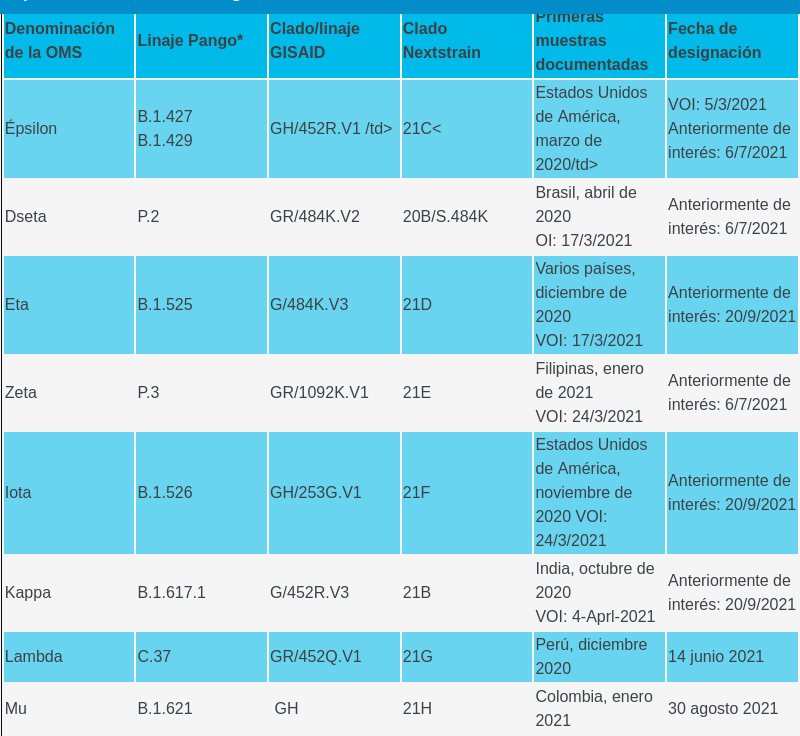
\includegraphics[width=\textwidth]{tabla variantes de interes.png}
    \caption{Variantes de Interés anteriormente en circulación. fuente: "Seguimiento de las variantes del SARS-CoV-2", OMS}
\end{figure*}

Tal y como se mencionó previamente en la introducción, uno de los motivos por lo que la pandemia del COVID-19 ha durado tanto tiempo es la constante evolución de nuevas variantes del virus original. Pese a que lo más común es que las mutaciones del virus no produzcan un cambio apreciable en ninguna característica del mismo, han aparecido variaciones a lo largo del tiempo que han demostrado ser más infecciosas que el virus original, más propensas a la hospitalización de la persona infectada, o incluso más resistente a las vacunas que se han desarrollado.

La OMS ha estado en investigación y reconocimiento de variantes desde enero del 2020, a pleno inicio de la pandemia, y ha generado un sistema simple de clasificación para estas en dos grandes grupos. 

\subsubsection*{Variantes de interés} son aquellas presentan que un cambio en su genoma que se ha demostrado o se prevé que afecte alguna de las características del virus de las que se mencionó anteriormente (Transmisibilidad, gravedad de enfermedad o resistencia a la respuesta inmune, entre otros); 

\subsubsection*{Variantes Preocupantes} son aquellas que la OMS clasifica como una Variante de Interés que además cumple con una o más de estas características en un grado que pueda ser significativo para la salud mundial: Aumento de Transmisibilidad, Aumento en la Virulencia o Disminución en la eficacia de metodos de prevención o detección.\cite{oms}

Actualmente solo existen 2 variantes de preocupación, y ninguna que sea de interés, que estén activamente en circulación, la variante Delta y la Variante Omicrón. La principal preocupación de estas variantes es su altísima transmisiblidad: tienen una de las tazas de contagio más altas que se ha detectado entre las variantes de COVID-19. El gran alivio que presentan, sin embargo, es su baja gravedad a la hora de infectar. Según lo que se mostró en la oleada de omicrón que afectó hace un tiempo a Chile y el mundo, la poca 'fuerza' que tiene esta variante al mostrar síntomas, sumado al esfuerzo vacunatorio de los países ha hecho que la necesidad de hospitalización disminuyera considerablemente respecto a la versión original del virus.

\subsubsection*{Omicrón}
Al igual que cualquier otra variante del COVID, Omicrón es compuesta por un número de linages y sublinages, siendo BA.1, BA.1.1 y BA.2 los más comunes. Lo que caracteríza esta variante, es que es la que se transmite con más facilidad entre todas las anteriores variantes de virus causantes del COVID-19, incluyendo incluso la variante Delta.

En general, sin embargo, la variante omicrón es mucho menos severa en cuanto a la gravedad de sus infecciones que otras variantes. Pese a que los datos dicten que la enfermedad generada por esta variante sea más ligera, alguna personas aún pueden ser propensas a desarrollar más complicaciones, necesitando hospitalización, e incluso generando el fallecimiento de otros. Incluso si muy pocas personas requiren hospitalización, sin embargo, la variante es tan infecciosa que estas pocas personas pueden llegar a ser grandes volúmenes de gente, capaces de sobrecargar el sistema de salud de un país.

Actualmente, el proceso vacunario sigue siendo el mejor sistema de protección para la gente que tiene COVID-19. Sin embargo, hay que recordar que estas vacunas son para prevenir enfermedades graves, más no son totalmente útiles para la infección y transmisión del virus. Una persona vacunada aún puede infectarse de Omicrón, y puede infectar a otros una vez finalizado su periodo latente.

Omicrón, y el resto de variantes, siguen siendo detectables por los métodos que se han utilizado hasta ahora, tanto PCR como Test de Antígenos.
